\chapter{Morphologie}
\label{sec:morphologie}

In diesem Kapitel werden einige Grundlagen der Morphologie besprochen.
Die Morphologie beschäftigt sich mit der äußeren Form von Wörtern und Wortformen in Zusammenhang mit ihren Merkmalen und Werten.
Dabei gibt es zwei Teilbereiche der Morphologie, die sich mit unterschiedlichen Relationen zwischen Wörtern beschäftigen.
Zunächst ist dabei die Beschreibung der Beziehungen zwischen den verschiedenen Formen eines Wortes -- die sogenannte \textit{Flexion} -- zu nennen.
Für die veränderlichen bzw.\ flektierbaren Wörter wird dabei erforscht, wie die Wortformen lexikalischer Wörter gebildet werden (\zB welche Endungen hinzutreten), und mit welchen Merkmalsänderungen diese Formbildungen einhergehen.
Beispielhaft für die Flexion sei hier die Form \textit{Wort-es} genannt, bei der die formale Kennzeichnung der Wortform das angefügte \textit{-es} ist, das mit der Setzung des Werts [\textsc{Kasus}: \textit{gen}] zusammenhängt.
Zweitens beschreibt die Morphologie aber auch produktive Beziehungen zwischen Wörtern, womit vor allem die Bildung neuer Wörter aus vorhandenen Wörtern gemeint ist.
Zum Beispiel ist \textit{täg-lich} offensichtlich ein aus dem Substantiv \textit{Tag} gebildetes Adjektiv.
Zwei weitere Beispiele sind die Bildung (\textit{der}) \textit{Lauf} (aus dem Verb \textit{lauf-en}) oder \textit{Haus-tür} aus \textit{Haus} und \textit{Tür}.
Die Beschreibung solcher Beziehungen ist die Aufgabe der \textit{Wortbildung}, die in Abschnitt~\ref{sec:flexionundwortbildung} eingeführt und in Kapitel~\ref{sec:wortbildung} ausführlich besprochen wird.

Dieses Kapitel führt in die Morphologie allgemein am Beispiel der Flexion ein und gibt zunächst in Abschnitt~\ref{sec:formenundihrestruktur} einen Überblick über Wortformen, ihre Funktionen und ihre interne Struktur.
In Abschnitt~\ref{sec:morphologischestrukturen} werden dann Formate zur Beschreibung morphologischer Strukturen eingeführt und in Abschnitt~\ref{sec:flexionundwortbildung} folgt schließlich eine Definition des Unterschieds von Flexion und Wortbildung.

\section{Formen und ihre Struktur}
\label{sec:formenundihrestruktur}

\subsection{Form und Funktion}
\label{sec:formundfunktion}

Die grundlegenden Fragen, die man sich in der Morphologie stellt, sind zwei scheinbar sehr einfache:
Welche Formen (im Sinne von Segmentfolgen) können Wörter haben?
Warum haben Wortformen und Bestandteile von Wortformen die Form, die sie haben?
In wissenschaftlichen Kontexten sind \textit{warum}-Fragen mit Vorsicht zu betrachten.
Die hier gestellte \textit{warum}-Frage ist keine Frage nach einer Ursache oder einem Sinn.
Ganz im Sinne von Abschnitt~\ref{sec:sprache} bezieht sich diese Frage auf ein bestimmtes Sprachsystem.
Man könnte die zweite Frage also präziser und bescheidener formulieren als:
Was ist der Stellenwert der Wortformen und ihrer Bestandteile innerhalb des Systems der untersuchten Sprache?
Dass diese Frage nicht völlig trivial ist, sieht man daran, dass es auch Sprachen gibt, die im Wesentlichen ohne Formveränderungen auskommen.
Das Chinesische ist ein Standardbeispiel für eine Sprache, in der im Grunde keine Flexion stattfindet.
Welche grammatische Funktion \zB ein Substantiv hat, ist in solchen Sprachen nicht an einer speziellen Kasusform abzulesen.
Nicht einmal Unterscheidungen wie Singular und Plural müssen gemacht werden.

Sich vorzustellen, die eigene Sprache könnte ohne die gewohnten grammatischen Kategorien funktionieren, ist üblicherweise sehr schwer.
Für viele Sprecher ist es \zB undenkbar, dass ein Sprachsystem wie das Deutsche ohne Flexion funktionieren würde.
Unter einer sprachpflegerischen Perspektive würde man eventuell sogar von einem \textit{Verlust der Ausdrucksmöglichkeiten} oder einer \textit{Verflachung} sprechen, wenn Flexionsendungen verloren gehen oder zusammenfallen.
Die Unterscheidung von Dativ und Genitiv hat für viele Sprecher in diesem Sinn einen hohen emotionalen Stellenwert.
Hier soll die Frage nach dem Stellenwert bzw.\ der Notwendigkeit der Flexion im Deutschen möglichst neutral und nicht emotional betrachtet werden.
Dazu ziehen wir das Englische hinzu.
Das Englische ist zwar eine dem Deutschen verwandte Sprache, weist aber strukturell große Unterschiede zum Deutschen auf.
Ein wichtiger Unterschied ist, dass es im Englischen bei den Nomina im Wesentlichen keine Differenzierung von Kasusformen mehr gibt.
Vergleichen wir nun einen deutschen Satz wie (\ref{ex:formundfunktion002}) mit dem englischen Satz in (\ref{ex:formundfunktion003}).

\begin{exe}
  \ex\label{ex:formundfunktion001}
  \begin{xlist}
    \ex\label{ex:formundfunktion002} Der Stürmer befördert den Ball ins Netz.
    \ex\label{ex:formundfunktion003} \gll The forward puts the ball into the net.\\
    der Stürmer befördert der Ball in das Netz\\
    \glt Der Stürmer befördert den Ball ins Netz.
  \end{xlist}
\end{exe}

Bezüglich der Reihenfolge der Satzteile und der Flexion ergeben sich nun von (\ref{ex:formundfunktion002}) ausgehend im Vergleich zu dem englischen Satz in (\ref{ex:formundfunktion003}) keine Unterschiede außer dem Fehlen der Akkusativ-Markierung bei \textit{den Ball}.\index{Flexion}
Das Englische zeigt also, dass Sprachsysteme offensichtlich auch ohne starke Flexionsmittel funktionieren.
\index{Kasus!Funktion}\index{Akkusativ}
Welche Funktion hat das System der Kasusmarkierungen also im Deutschen, wenn das Englische offensichtlich auch ohne ein solches System auskommt?%
\footnote{Das Englische ist hier nur exemplarisch.
Gleiches könnte man \zB auch über die romanischen Sprachen (wie Französisch oder Italienisch) oder viele andere Sprachen sagen.}
Diese Frage kann man nur mit Blick auf den Gesamtzusammenhang des Sprachsystems beantworten.
Sehen wir uns dazu weitere Beispiele an.

\begin{exe}
  \ex \label{ex:formundfunktion004}
  \begin{xlist}
    \ex{\label{ex:formundfunktion005} Der Stürmer foulte den Verteidiger.}
    \ex{\label{ex:formundfunktion006} Den Verteidiger foulte der Stürmer.}
    \ex\label{ex:formundfunktion007} \gll The forward fouled the defender.\\
    der Stürmer foulte der Verteidiger\\
    \glt Der Stürmer foulte den Verteidiger.
    \ex\label{ex:formundfunktion008} \gll The defender fouled the forward.\\
    der Verteidiger foulte der Stürmer\\
    \glt Der Verteidiger foulte den Stürmer.
  \end{xlist}
\end{exe}

Die deutschen Sätze (\ref{ex:formundfunktion005}) und (\ref{ex:formundfunktion006}) sind eindeutig zu interpretieren und bedeuten das Gleiche, obwohl Subjekt und Objekt in umgekehrter Reihenfolge vorkommen.%
\footnote{Was unter den Begriffen \textit{Subjekt} und \textit{Objekt} zu verstehen ist, wird erst in Kapitel~\ref{sec:relationenundpraedikate} ausführlich besprochen.
Im Prinzip ist das Subjekt die Nominativ-Ergänzung des Verbs und die Objekte die anderen kasusregierten Ergänzungen des Verbs.}
In beiden Fällen ist der Stürmer derjenige, der den Verteidiger gefoult hat.\index{Subjekt}\index{Objekt}
Was bedeuten die englischen Sätze (\ref{ex:formundfunktion007}) und (\ref{ex:formundfunktion008}), in denen auch lediglich Subjekt und Objekt die Plätze tauschen?
Die Interpretation dreht sich in (\ref{ex:formundfunktion008}) um, so dass eine Situation beschrieben wird, in der der Verteidiger den Stürmer gefoult hat.

Die strukturellen Auslöser für diesen Effekt sind schnell gefunden.
Obwohl das Subjekt im Deutschen vor dem Objekt stehen kann, muss dies nicht unbedingt der Fall sein, vgl.\ (\ref{ex:formundfunktion006}).
Wenn von dieser Stellung abgewichen wird und das Objekt vor dem Subjekt steht, ermöglichen die Kasusformen (hier an den Artikeln \textit{der} und \textit{den} zu erkennen) dennoch eine Identifizierung des Subjekts und des Objekts.
Wenn die Kasusmarkierung wie im Englischen entfällt, schränken sich die Möglichkeiten der Umstellung ein, da zur Identifizierung der Funktion (Subjekt oder Objekt) nur noch die Reihenfolge der Satzglieder herangezogen werden kann.
Anders gesagt ermöglichen die Mittel der Kasusflexion im Deutschen eine freiere Wortstellung als im Englischen, und die verschiedenen Wortstellungstypen können dadurch ihrerseits andere Funktionen markieren (vgl.\ Kapitel~\ref{sec:saetze}).

Sogar innerhalb des Deutschen kann man dies illustrieren, wenn man \zB feminine Substantive auswählt.
Weder das Substantiv noch der bestimmte Artikel haben hier im Singular unterschiedliche Formen für Nominativ und Akkusativ.

\begin{exe}
  \ex \label{ex:formundfunktion009}
  \begin{xlist}
    \ex{Die Stürmerin foulte die Verteidigerin.}
    \ex{Die Verteidigerin foulte die Stürmerin.}
  \end{xlist}
\end{exe}

Als Folge davon sind ähnliche Umstellungsmöglichkeiten wie in (\ref{ex:formundfunktion001}) hier nicht gegeben.%
\footnote{Diese Aussage stimmt nicht ganz.
Mit dem richtigen Kontext und besonderer Betonung kann man auch hier beide Lesarten erzwingen.
Trotzdem muss festgestellt werden, dass durch das Fehlen der Kasusmarkierung im Femininum erhebliche Einschränkungen der Verfügbarkeit der Lesarten bestehen.}
Die Sätze in (\ref{ex:formundfunktion009}) haben unterschiedliche Bedeutung.
Die Markierung bestimmter grammatischer Merkmale und Funktionen (die wiederum die Interpretation von Sätzen erst ermöglichen) ist also auf verschiedene formale und strukturelle Mittel verteilt, zum Beispiel auf die Flexion und die Wortstellung.
Wir können vermuten, dass in jedem Sprachsystem die Mittel auf eine in irgendeiner Hinsicht optimale Weise verteilt sind, so dass im Regelfall die Gesamtform eines Satzes keine oder wenig Doppeldeutigkeiten zulässt, die die Kommunikation negativ beeinflussen.

Abschließend sei darauf verwiesen, dass als Mittel zur Markierung grammatischer Funktionen nicht nur Flexion und Wortstellung infragekommen.
Betrachten wir die deutschen Beispiele in (\ref{ex:formundfunktion010}) und (\ref{ex:formundfunktion011}).

\begin{exe}
  \ex \label{ex:formundfunktion010}
  \begin{xlist}
    \ex{Wir laufen in den Wald.}
    \ex{Wir laufen im Wald.}
  \end{xlist}
  \ex \label{ex:formundfunktion011}
  \begin{xlist}
    \ex\gll I enjoy being out in the woods.\\
    Ich genieße seiend draußen in der Wald\\
    \glt Ich bin gerne im Wald.
    \ex\gll Tomorrow, {we'll} go out into the woods.\\
    morgen {wir.werden} gehen raus in der Wald\\
    \glt Morgen gehen wir in den Wald.
  \end{xlist}
\end{exe}

\index{Präposition!Wechsel--}\index{Akkusativ}\index{Dativ}

Präpositionen wie \textit{in} treten im Deutschen mit zwei verschiedenen Kasus auf (Akkusativ und Dativ) und werden daher auch \textit{Wechselpräpositionen} genannt.
Ob ein Ortswechsel (\textit{in den Wald}) oder ein eher statischer Ort (\textit{im Wald}) beschrieben wird, hängt dabei vom Kasus der folgenden Nomina ab.
Dieser Unterschied wird \zB im Englischen in einigen Fällen lexikalisch, nämlich mittels verschiedener Präpositionen ausgedrückt, \textit{into} für die Richtung bzw.\ das Ziel und \textit{in} für den Ort.
Natürlich haben wir damit nicht alle möglichen Mittel benannt, grammatische Funktionen zu markieren.
Auf jeden Fall haben wir aber herausgestellt, in welchem Gesamtkontext die Morphologie ihren Platz hat.
Die darauf basierende Definition~\ref{def:morphologie} schließt diesen Abschnitt ab.

\Definition{Morphologie}{\label{def:morphologie}%
Die \textit{Morphologie} beschreibt die Regularitäten der Wortformenbildung (Flexion) und der Wortbildung einschließlich der grammatischen und lexikalischen Funktionen, die durch sie markiert werden.
\index{Morphologie}
}

Um die morphologischen Besonderheiten des Deutschen beschreiben zu können, benötigen wir als nächstes eine Redeweise über Wortformen und ihre Bestandteile.
Eine solche wird in den Abschnitten~\ref{sec:morphe} und~\ref{sec:woerterwortformenundstaemme} eingeführt.

\subsection{Morphe}
\label{sec:morphe}

Schon in Abschnitt~\ref{sec:definitionsprobleme} (genauer Seite~\pageref{arbref:9234645}) wurde von Wortbestandteilen als Einheiten gesprochen, weil zum Beispiel für \textit{-es} in Genitiv-Wortformen wie \textit{Staat-es} offensichtlich eigene Regularitäten bezüglich der Kombinationsmöglichkeiten gelten.%
\footnote{Wir geben Segmentfolgen der Lesbarkeit halber prinzipiell mit ihrem orthographischen Korrelat an, sofern sich dadurch keine Ungenauigkeiten in der Darstellung ergeben.}
Zudem erscheint es auch plausibel, anzunehmen, die Endungen (wie \textit{-es}) wären Träger bestimmter Merkmale bzw.\ der Werte (hier \textsc{Kasus} und \textsc{Numerus}), die an vollständige Wortformen wie \textit{Staat-es} weitergegeben werden.
In solch einer Denkweise trüge also \textit{-es} selber die Spezifikation [\textsc{Kasus}: \textit{gen}, \textsc{Numerus}: \textit{sg}] mit sich.
Wir wollen hier allerdings im Weiteren etwas abgeschwächt davon sprechen, dass diese Wortbestandteile nur die entsprechenden Merkmale und Werte \textit{markieren}, und nicht, dass sie Merkmale und Werte \textit{tragen}.
Mit \textit{markieren} ist hier gemeint, dass sie dem Hörer signalisieren, dass die Wortform bestimmte Werte hat.
Diese abgeschwächte Auf"|fassung ist für die Analyse der Formen des Deutschen überwiegend zielführender, was in Kapitel~\ref{sec:nominalflexion} und Kapitel~\ref{sec:verbalflexion} weiter thematisiert wird.%
\footnote{Eine Abgrenzung zu der weit verbreiteten Terminologie der \textit{Morpheme} und \textit{Allomorphe} findet sich in Vertiefung~\ref{vert:morphemeallomorphe} auf Seite~\pageref{vert:morphemeallomorphe}.}
Zunächst soll für die Wortbestandteile der Begriff des \textit{Morphs} mit Definition~\ref{def:morph} eingeführt werden.

\Definition{Morph}{\label{def:morph}%
Ein \textit{Morph} ist jede Segmentfolge innerhalb einer Wortform, die mit mindestens einer Markierungsfunktion verknüpft ist.
\index{Morph}
}

Der Begriff \textit{Markierungsfunktion} muss mit Definition~\ref{def:markfunk} ebenfalls explizit eingeführt werden.

\Definition{Markierungsfunktion}{\label{def:markfunk}%
Ein Morph hat eine \textit{Markierungsfunktion} genau dann, wenn durch seine Anwesenheit die möglichen (lexikalischen und grammatischen) Merkmale und\slash oder die möglichen Merkmalswerte, die die Wortform haben kann, eingeschränkt werden.
\index{Markierungsfunktion}
}

Die Markierungsfunktion von Wortbestandteilen wird anhand der Beispiele (\ref{ex:morphe012}) bis (\ref{ex:morphe014}) demonstriert.

\Enl

\begin{exe}
  \ex \label{ex:morphe012}
  \begin{xlist}
    \ex{(der) Berg}
    \ex{(den) Berg}
    \ex{(dem) Berg}
    \ex{(des) Berg-es}
    \ex{(die) Berg-e}
    \ex{(der) Berg-e}
  \end{xlist}
  \ex \label{ex:morphe013}
  \begin{xlist}
    \ex{(der) Mensch}
    \ex{(den) Mensch-en}
    \ex{(dem) Mensch-en}
    \ex{(des) Mensch-en}
    \ex{(die) Mensch-en}
    \ex{(der) Mensch-en}
  \end{xlist}

  \ex \label{ex:morphe014}
  \begin{xlist}
    \ex{(ich) kauf-e}
    \ex{(du) kauf-st}
    \ex{(wir) kauf-en}
    \ex{(sie) kauf-en}
  \end{xlist}
\end{exe}

Die in (\ref{ex:morphe012}) bis (\ref{ex:morphe014}) mit \textit{-} abgetrennten Morphe erfüllen Definition~\ref{def:markfunk} eindeutig.
Die Wortform \textit{Berg-es} ist durch die Anwesenheit des Morphs \textit{-es} auf ganz bestimmte Merkmale eingeschränkt, nämlich mindestens [\textsc{Kasus}: \textit{gen}, \textsc{Numerus}: \textit{sg}].
\label{abs:morphe015}Auch wenn für \textit{Berg-e} keine ganz eindeutige Einschränkung für die Werte von \textsc{Kasus} und \textsc{Numerus} festgestellt werden kann, so kann diese Wortform \zB auf keinen Fall [\textsc{Kasus}: \textit{nom}, \textsc{Numerus}: \textit{sg}] sein.\index{Kasus}\index{Numerus}
In (\ref{ex:morphe013}) sind Wortformen von \textit{Mensch} aufgelistet.
In diesem Fall hat nur der Nominativ Singular die Form \textit{Mensch}, alle anderen Formen lauten \textit{Mensch-en}.
Auch hier reduziert die Anwesenheit von \textit{-en} die Möglichkeiten für die Werte der \textsc{Kasus}- und \textsc{Numerus}-Merkmale auf alles außer [\textsc{Kasus}: \textit{nom}, \textsc{Numerus}: \textit{sg}].
\index{Wort!Bedeutung}
Ganz ähnlich verhält es sich in (\ref{ex:morphe014}) mit \textit{kauf-e}, \textit{kauf-st} usw.
Die Morphe \textit{-e}, \textit{-st} und \textit{-en} schränken die möglichen \textsc{Person}- und \textsc{Numerus}-Werte teilweise eindeutig, teilweise mehrdeutig ein.

Leicht übersieht man (aus Gründen, die in Abschnitt~\ref{sec:woerterwortformenundstaemme} noch eine Rolle spielen werden), dass auch \textit{Berg}, \textit{Mensch} und \textit{kauf} eine Markierungsfunktion haben und damit auch Morphe sind.
Diese Morphe schränken zum Beispiel die Wortklasse der Wortform und vor allem ihre Bedeutung ein.
Im Fall von Morphen wie \textit{Berg} und \textit{Mensch} ist es sicherlich unstrittig, dass sie eine Bedeutung haben, egal welche Theorie von Bedeutung man zugrundelegt.
Wo es die Überlegungen vereinfacht, soll deshalb in Zukunft die Bedeutung als ein Merkmal hinzugezogen werden.
Dabei wird die Bedeutung hier nicht analysiert, sondern einfach bezeichnet wie in (\ref{ex:morphe016}).

\begin{exe}
  \ex\label{ex:morphe016}
  \begin{xlist}
    \ex{Berg $=$ [\textsc{Bedeutung}: \textit{berg}, \ldots]}
    \ex{Mensch $=$ [\textsc{Bedeutung}: \textit{mensch}, \ldots]}
  \end{xlist}
\end{exe}

Damit haben also die Morphe \textit{Berg} und \textit{Mensch} auch eine Markierungsfunktion bezüglich des Merkmals \textsc{Bedeutung}.
Mit einem indirekteren Bezug auf die Bedeutung kann man sagen, dass Morphe wie \textit{Berg} die Zugehörigkeit der Wortform zu einem bestimmten lexikalischen Wort markieren.

\subsection{Wörter, Wortformen und Stämme}
\label{sec:woerterwortformenundstaemme}

\index{Wort}

Die Beziehung zwischen Wort und Wortform wurde bereits in Abschnitt~\ref{sec:woerterundwortformen} hinreichend charakterisiert.
Die Definitionen~\ref{def:wortform} (Seite~\pageref{def:wortform}) und \ref{def:wort} (Seite~\pageref{def:wort}) definieren die \textit{Wortform} (bzw.\ das \textit{syntaktische Wort}) als die konkrete, in ihren Merkmalswerten maximal spezifische Einheit, die ggf.\ eine besondere Flexionsform hat.
Das (\textit{lexikalische}) \textit{Wort} ist hingegen die abstrakte Repräsentation aller im Paradigma vertretenen Wortformen, bei der die Werte für Merkmale nur dann spezifiziert sind, wenn sie in allen zugehörigen Wortformen gleich sind.

An anderer Stelle, nämlich in Abschnitt~\ref{sec:wortakzentimdeutschen} (genauer Seite~\pageref{abs:wortakzentimdeutschen170}) haben wir uns bereits vorläufig auf den \textit{Stamm} bezogen.
An dem genannten Ort war es nicht möglich, eine besonders exakte Definition des Stamms zu geben.
Es wurde aber angedeutet, dass der Stamm die in allen Wortformen eines Wortes unveränderliche Segmentfolge sei.
Um zu überprüfen, ob eine solche Definition dauerhaft tragfähig ist, sehen wir uns zunächst wieder einige Beispiele an.

\begin{exe}
  \ex \label{ex:woerterwortformenundstaemme017}
  \begin{xlist}
    \ex{(ich) kauf-e\\
      (du) kauf-st\\
      (es) kauf-t }
    \ex{(ich) kauf-te\\
      (du) kauf-te-st\\
      (es) kauf-te }
  \end{xlist}
  \ex \label{ex:woerterwortformenundstaemme018}
  \begin{xlist}
    \ex{(ich) nehm-e\\
      (du) nimm-st\\
      (es) nimm-t\\
      (wir) nehm-en }
    \ex{(ich) nahm\\
      (du) nahm-st\\
      (es) nahm }
  \end{xlist}
  \ex \label{ex:woerterwortformenundstaemme019}
  \begin{xlist}
    \ex{(ich) geh-e\\
      (du) geh-st\\
      (es) geh-t }
    \ex{(ich) ging\\
      (du) ging-st\\
      (es) ging }
  \end{xlist}
  \ex \label{ex:woerterwortformenundstaemme020}
  \begin{xlist}
    \ex{(die) Sau\\
      (der) Sau\\
      (die) Säu-e\\
      (den) Säu-en }
  \end{xlist}
\end{exe}

(\ref{ex:woerterwortformenundstaemme017}) bis (\ref{ex:woerterwortformenundstaemme019}) gehören zum \textsc{Tempus}-\textsc{Person}-\textsc{Numerus}-Paradigma der Verben, und (\ref{ex:woerterwortformenundstaemme020}) gehört zum \textsc{Kasus}-\textsc{Numerus}-Paradigma der Substantive.
Trotzdem gibt es nicht in allen Fällen eine eindeutige, sich nicht verändernde Segmentfolge.

In (\ref{ex:woerterwortformenundstaemme017}) ist \textit{kauf} eindeutig ein nicht veränderlicher Bestandteil, wobei alle Formen des Präteritums (der sogenannten \textit{Vergangenheit}) \textit{kauf-te} beinhalten, also der feste Bestandteil mit einem \textit{-te} erweitert ist.
In (\ref{ex:woerterwortformenundstaemme018}) ändert sich der Vokal von /\textipa{e}/ zu /\textipa{I}/ in der zweiten und dritten Person des Singulars (\textit{nehm} zu \textit{nimm}).
Im Präteritum enthalten alle Formen \textit{nahm}, der Vokal wechselt also zu /\textipa{a}/.
In (\ref{ex:woerterwortformenundstaemme019}) gehen die Veränderungen im Präteritum so weit, dass neben der Vokaländerung sogar ein auslautender Konsonant hinzutritt und statt /\textipa{ge}/ \textit{geh} die Folge /\textipa{gIng}/ \textit{ging} eintritt.
(\ref{ex:woerterwortformenundstaemme020}) zeigt schließlich eine ähnliche Vokalveränderung im Substantiv-Paradigma mit den Stämmen \textit{Sau} /\textipa{z\t{aO}}/ und \textit{Säu} /\textipa{z\t{O\oe}}/.
Es gibt also nicht in jedem Fall genau einen unveränderlichen Bestandteil im Paradigma eines lexikalischen Wortes, sondern öfter auch mehrere verschiedene.
Daher definieren wir den \textit{Wortstamm} in Definition~\ref{def:stamm}.

\Definition{Stamm}{\label{def:stamm}%
Ein \textit{Stamm} oder \textit{Wortstamm} ist der Teil einer Wortform, der die lexikalische Markierungsfunktion trägt.
In den Formen ihres Paradigmas können Wörter verschiedene Stämme haben.
\index{Stamm}
}
\index{Markierungsfunktion!lexikalisch}

\Stretch[-0.5]

Mit einer \textit{lexikalischen Markierungsfunktion} ist hier gemeint, dass der Stamm die Zugehörigkeit der Wortform, in der er vorkommt, zu einem bestimmten lexikalischen Wort markiert.
Einfacher gesagt ist der Stamm der Teil der Wortform, an dem man das Wort erkennt.
An den Wortstamm treten typischerweise die Flexionsaffixe, vgl.\ die Abschnitte~\ref{sec:linearebeschreibung} und~\ref{sec:flexionundwortbildung}.

Im Deutschen werden für bestimmte Formen in Paradigmen (oder in bestimmten Wortbildungen, vgl.\ Kapitel~\ref{sec:wortbildung}) unterschiedliche Stämme zugrundegelegt.
Typisch ist zum Beispiel bei den sogenannten \textit{starken Verben} (vgl.\ Abschnitt~\ref{sec:verbalflexion}), dass das Präsens wie (\textit{ich}) \textit{bitt-e}, das Präteritum wie (\textit{ich}) \textit{bat} und die Partizipien wie (\textit{ich habe}) \textit{ge-bet-en} einen Stamm mit jeweils unterschiedlichem Vokal aufweisen.
Man nennt dieses Phänomen den \textit{Ablaut} und spricht auch vom \textit{Präsensstamm}, einem \textit{Präteritalstamm} und einem \textit{Partizipialstamm}.
Zur Unterscheidung dieses Mittels der Stammbildung im Deutschen vom Umlaut geht es in Abschnitt~\ref{sec:umlautundablaut}.

\subsection{Umlaut und Ablaut}
\label{sec:umlautundablaut}

\Enl[2]

In Übung \ref{exc:phonologie02} auf Seite~\pageref{exc:phonologie02} wurde bereits nach der phonologischen Beschreibung des Umlauts gefragt.
Die Paare von nicht umgelautetem und umgelautetem Vokal sind die in (\ref{ex:umlautundablaut021}).

\begin{exe}
  \ex\label{ex:umlautundablaut021}
  \begin{xlist}
    \ex{/\textipa{u}/ -- /\textipa{y}/ (Fuß, Füße)}
    \ex{/\textipa{U}/ -- /\textipa{Y}/ (Genuss, Genüsse)}
    \ex{/\textipa{o}/ -- /\textipa{\o}/ (rot, röter)}
    \ex{/\textipa{O}/ -- /\textipa{\oe}/ (Koffer, Köfferchen)}
    \ex{/\textipa{a}/ -- /\textipa{E}/ (Schlag, Schläge)}
    \ex{/\textipa{\u{a}}/ -- /\textipa{\u{E}}/ (Bach, Bäche)}
  \end{xlist}
\end{exe}

\Np

\begin{figure}[!htpb]
  \centering
  \begin{tikzpicture}[scale=3.5,baseline=default]
  \large
  \tikzset{
    vowel/.style={fill=white, anchor=mid, text depth=0ex, text height=1ex},
    vowelgespannt/.style={circle,fill=gray!30, anchor=mid, text depth=0ex, text height=1ex,minimum size=4ex},
    dot/.style={circle,fill=black,minimum size=0.4ex,inner sep=0pt,outer sep=-1pt},
  }

  \coordinate (hf) at (0,2); % high front
  \coordinate (hb) at (2,2); % high back
  \coordinate (lf) at (1,0); % low front
  \coordinate (lb) at (2,0); % low back
  \def\V(#1,#2){barycentric cs:hf={(3-#1)*(2-#2)},hb={(3-#1)*#2},lf={#1*(2-#2)},lb={#1*#2}}

  % Chart key (vorne -- hinten).
  \draw [{Latex[round]}-] (\V (-.25,0)) -- (\V (-.25,.5)) node[above left] {\footnotesize vorne};
  \draw [-{Latex[round]}] (\V (-.25,1.5)) -- (\V (-.25,2)) node[above left] {\footnotesize hinten};
  \path (\V (-.25,1)) node[above] {\footnotesize zentral};

  % Chart key (hoch -- tief).
  \draw [{Latex[round]}-] (\V (0,-.25)) -- +(270:.5cm) node[above right,rotate=90] (vokaltrapez1) {\footnotesize hoch};
  \draw [{Latex[round]}-] (\V (3,-2.5)) -- +(270:-.5cm) node[above left,rotate=90] (vokaltrapez2) {\footnotesize tief};
  \path (\V (1.5,-1)) node[above,rotate=90] {\footnotesize mittel};

  % Grid.
  \draw [gray, thick] (\V(0,0)) -- (\V(0,2));
  \draw [gray, thick] (\V(3,0)) -- (\V(3,2));
  \draw [gray, thick] (\V(0,0)) -- (\V(3,0));
  \draw [gray, thick] (\V(0,2)) -- (\V(3,2));

  % Vowels.
  \path (\V (0,2))     node[vowelgespannt] (u)   {u};
  \path (\V(0,0))      node[vowelgespannt] (y)   {y};
  \path (\V (0.5,1.5)) node[vowel]         (uu)  {ʊ};
  \path (\V(0.5,0.5))  node[vowel]         (yy)  {ʏ};
  \path (\V (1,2))     node[vowelgespannt] (o)   {o};
  \path (\V(1.25,0))   node[vowelgespannt] (oe)  {ø};
  \path (\V(3,1))      node[vowelgespannt] (a)   {a};
  \path (\V(2,0))      node[vowelgespannt] (ee)  {ɛ};
  \path (\V(2.5,1))    node[vowel]         (aa)  {ă};
  \path (\V(1.65,0.5)) node[vowel]         (eee) {ɛ̆};
  \path (\V (1.5,1.4)) node[vowel]         (oo)  {ɔ};
  \path (\V(1.4,0.5))  node[vowel]         (oee) {œ};

  \path (u)  edge [-{Latex[round]}, bend left=10]  (y);
  \path (uu) edge [-{Latex[round]}, bend left=10]  (yy);
  \path (o)  edge [-{Latex[round]}, bend right=10] (oe);
  \path (oo) edge [-{Latex[round]}, bend right=5]  (oee);
  \path (aa) edge [-{Latex[round]}, bend right=10] (eee);
  \path (a)  edge [-{Latex[round]}, bend left=10]  (ee);
  \end{tikzpicture}
  \caption{Umlaut im phonologischen Vokaltrapez}
  \label{fig:umlautundablaut022}
  \index{Vokaltrapez}
\end{figure}

Die Auf"|lösung erfolgt jetzt, indem die nicht umgelauteten und die zugehörigen umgelauteten einfachen Vokale in Abbildung~\ref{fig:umlautundablaut022} im (phonologischen) Vokaltrapez dargestellt werden (vgl.\ auch Abbildung~\ref{fig:gespanntheitbetonungundlaenge019} auf Seite~\pageref{fig:gespanntheitbetonungundlaenge019}).
An dieser Darstellung ist leicht zu erkennen, dass alle umgelauteten Vokale [\textsc{Lage}: \textit{vorne}] sind.
Alle anderen Merkmale (einschließlich \textsc{Gespannt}) sind bei den nicht-umge\-laute\-ten und den zugehörigen umgelauteten Vokalen gleich spezifiziert.
Man spricht daher auch von \textit{Frontierung}.
Der Umlaut lässt sich also als \textit{morphologisch bedingte phonologische Regularität} beschreiben.
\textit{Regularität} bedeutet hier, dass zu jedem umlautfähigen Vokal immer eindeutig bestimmbar ist, was der zugehörige Umlautvokal ist.
Prinzipiell nicht am Umlaut beteiligt sind /\textipa{i I e @ 5}/.
Der Umlaut von /\textipa{\t{aO}}/ zu /\textipa{\t{O\oe}}/ ist etwas schwieriger zu beschreiben.
Das zweite Glied im Diphthong wird aber auch hierbei frontiert, also /\textipa{O}/ zu /\textipa{\oe}/.
Definition~\ref{def:umlaut} fasst zusammen.

\Enl

\Definition{Umlaut}{\label{def:umlaut}%
Der \textit{Umlaut} ist eine systematische, morphologisch bedingte Veränderung der Vokalqualität, nämlich eine \textit{Frontierung}.
Der Qualitätsunterschied ist phonologisch regulär (also vorhersagbar).
\index{Umlaut}
}

Der Ablaut stellt sich gänzlich anders dar.
Nehmen wir dazu einige der sogenannten \textit{Ablautreihen} als Beispiele hinzu, wobei die Orthographie in der Gewissheit verwendet wird, dass die korrespondierenden Segmente klar rekonstruierbar sind.%
\footnote{Terminologisch ist der Begriff \textit{Ablaut} auf ein bestimmtes in der deutschen bzw.\ germanischen Sprachgeschichte begründetes Phänomen reserviert.
Einige ähnliche Vokalveränderungen bei den sogenannten \textit{starken Verben} haben historisch andere Ursachen.
In Kapitel~\ref{sec:verbalflexion} (besonders Abschnitt~\ref{sec:unterklassen}) wird daher allgemeiner von \textit{Vokalstufen} statt \textit{Ablautstufen} gesprochen.}

\Stretch[0.5]

\begin{exe}
  \ex\label{ex:umlautundablaut023}
  \begin{xlist}
    \ex{werb-e, warb, ge-worb-en}
    \ex{schwing-e, schwang, ge-schwung-en}
    \ex{schwimm-e, schwamm, ge-schwomm-en}
    \ex{lauf-e, lief, ge-lauf-en}
  \end{xlist}
\end{exe}

\Stretch[0.5]

Ohne eine detaillierte Analyse der Merkmale der betroffenen Vokale durchzuführen, kann man leicht sehen, dass hier keine einheitliche phonologische Beschreibung möglich ist.
Schon dass \textit{i -- a -- u} und \textit{i -- a -- o} nebeneinander existieren, zeigt, dass kein simpler phonologischer Prozess für den Ablaut verantwortlich sein kann.
Es ist zwar nicht richtig, hier von \textit{unregelmäßigen Bildungen} zu sprechen, weil es eine begrenzte (nicht beliebige) Zahl von Ablautreihen gibt.
Dennoch muss zu jedem starken Verb zumindest das Muster der Ablautreihe lexikalisch abgespeichert werden, um die Stämme richtig bilden zu können.
Diese Erkenntnis führt direkt zu Definition~\ref{def:ablaut}.

\Stretch

\Definition{Ablaut}{\label{def:ablaut}%
Der \textit{Ablaut} ist ein systematischer, morphologisch bedingter Unterschied der Vokalqualität in Wortstämmen.
Der Qualitätsunterschied ist nicht phonologisch regulär (also nicht vorhersagbar), sondern folgt einer größeren Menge von verschiedenen \textit{Ablautmustern} (auch: \textit{Ablautreihen}).
\index{Ablaut}
}

\Stretch[0.5]

Die allgemeine Diskussion der Morphologie ist hier vorerst abgeschlossen.
In Abschnitt~\ref{sec:morphologischestrukturen} folgt noch eine kurze Darstellung bestimmter Arten, morphologische Strukturen zu beschreiben.

\Np

\Zusammenfassung{%
In der Morphologie behandeln wir die Form von lexikalischen und syntaktischen Wörtern in Abhängigkeit von ihren Merkmalen und Werten.
Dabei sind Morphe die zentralen Bausteine, aus denen Wortformen aufgebaut werden, und die Markierungsfunktionen haben.
Der Stamm markiert die Zugehörigkeit zu einem bestimmten lexikalischen Wort.
Während der Umlaut eine reguläre morphologisch bedingte Frontierung von Vokalen darstellt, handelt es sich beim Ablaut um einen nicht vorhersagbaren Vokalwechsel.
}

\Stretch

\section{Morphologische Strukturen}
\label{sec:morphologischestrukturen}

\Stretch[0.5]

\subsection{Lineare Beschreibung}
\label{sec:linearebeschreibung}

Wir haben bis hierher die \textit{Wortform} (konkret vorkommende Form), das \textit{lexikalische Wort} (Abstraktion von paradigmatisch zusammengehörenden Wortformen), das \textit{Morph} (Konstituente einer Wortform) und den \textit{Stamm} (Morph mit lexikalischer Markierungsfunktion) als zentrale Begriffe eingeführt.
Jede Wortform muss im Normalfall mindestens einen Stamm enthalten, da eine Wortform immer einen lexikalischen Kern braucht, ohne den die Zuordnung der Wortform zu einem lexikalischen Wort nicht möglich wäre.

Bezüglich der zusätzlichen Morphe einer Wortform (also die Nicht-Stämme unter den Morphen) gibt es eine nützliche Terminologie, die ein präziseres Reden über die Struktur von Wortformen ermöglicht.
Es folgen jeweils einige Beispiele und die entsprechenden Definitionen bzw.\ Erläuterungen.

\Stretch[0.5]

\begin{exe}
  \ex\label{ex:linearebeschreibung024}
  \begin{xlist}
    \ex{Un-ding}
    \ex{(ich) ver-misch(-e)}
  \end{xlist}
  \ex\label{ex:linearebeschreibung025}
  \begin{xlist}
    \ex{(ich) leb-e}
    \ex{Gleich-heit}
  \end{xlist}
  \ex\label{ex:linearebeschreibung026}{Ge-red-e}
\end{exe}

\Stretch[0.5]

In (\ref{ex:linearebeschreibung024}) -- (\ref{ex:linearebeschreibung026}) treten jeweils Morphe, die keine Stämme sind, zu einem Stamm hinzu.
Solche Morphe nennt man allgemein \textit{Affixe}, vgl.\ Definition~\ref{def:affix}.

\Definition{Affix}{\label{def:affix}%
Ein \textit{Affix} ist ein Morph mit einer nicht-lexikalischen Markierungsfunktion, das nicht alleine, sondern nur in Verbindung mit einem Stamm auftreten kann.
\index{Affix}
}

\index{Präfix}
\index{Suffix}
\index{Zirkumfix}

Bezüglich der Position der Affixe innerhalb der Wortform lassen sich drei Typen von Affixen ausmachen.
In (\ref{ex:linearebeschreibung024}) stehen die Affixe \textit{Un}- und \textit{ver}- vor dem Stamm, weswegen sie \textit{Präfixe} (im weiteren Sinn) genannt werden.%
\footnote{In Kapitel~\ref{sec:wortbildung} werden die spezielleren Begriffe des \textit{Verbalpräfixes} und der \textit{Verbpartikel} eingeführt, die beide Präfixe i.\,w.\,S.\ sind.}
In (\ref{ex:linearebeschreibung025}) stehen die Affixe -\textit{e} und -\textit{heit} nach dem Stamm und werden als \textit{Suffixe} bezeichnet.
In (\ref{ex:linearebeschreibung026}) wiederum wird der Stamm umgeben von einem Präfix und einem Suffix, die im Prinzip zusammengehören, also \textit{Ge-~-e}.
In einem solchen Fall spricht man von einem \textit{Zirkumfix}.
Bisher trennen wir alle Arten von Affixen mit einem einfachen - ab (eine weitere Differenzierung dieser Notation findet sich in Kapitel~\ref{sec:wortbildung}).
Affixe werden von nun an (im Gegensatz zu Stämmen) mit diesem Bindestrich angegeben, wobei die Position des Bindestrichs anzeigt, ob es sich um ein Präfix (\textit{Un}-), ein Suffix (-\textit{heit}) oder ein Zirkumfix (\textit{Ge-~-e}) handelt.
Wenn eines dieser Affixe immer den Umlaut auslöst (s.\ Abschnitt~\ref{sec:umlautundablaut}), dann wird statt des Strichs die Tilde \char`~\ verwendet, also \zB \mbox{\textit{\char`~ chen}} (vgl.\ \textit{Bäum-chen}).

Die in diesem Abschnitt eingeführten Begriffe beschreiben die Konstituenten bezüglich ihrer linearen Abfolge.
Um hierarchische Strukturen in der Morphologie zu beschreiben, benötigt man ein anderes Strukturformat, das kurz in Abschnitt~\ref{sec:strukturformat} vorgestellt wird.

\subsection{Strukturformat}
\label{sec:strukturformat}

Eine Form wie (\textit{wir}) \textit{schick-te-n} können wir so beschreiben, dass zunächst das Suffix \textit{-te} an den Stamm \textit{schick} angeschlossen wird, und dann das Suffix \textit{-n} hinzutritt.
Diese Reihenfolge sollte plausibel erscheinen, weil so die Form sozusagen von innen nach außen aufgebaut werden kann.
Außerdem ist das \textit{-te} in allen Formen des Präteritums dieses Verbs vorhanden (vgl.\ (\textit{ich}) \textit{schick-te} usw.), weshalb durchaus anzunehmen ist, dass hier eine hierarchische Struktur vorliegt und dass \textit{-te} eine Konstituente mit dem Stamm bildet, die dann mit dem Suffix \textit{-n} die nächste Konstituente bildet.
Solche hierarchischen Strukturen lassen sich durch Baumdiagramme gut abbilden, s.\ Abbildung~\ref{fig:strukturformat027}.\index{Baumdiagramm}
Die eckigen Klammern zeigen an, dass es sich um eine nicht vollständige Struktur handelt.
Eine [Wortform] ist also eine Wortform, der noch Flexionsaffixe fehlen.%
\footnote{Warum hier \textit{-te} und \textit{-n} nacheinander angefügt werden, wird in Abschnitt~\ref{sec:verbaleflexion} begründet.}

\begin{figure}[!htbp]
  \centering
  \begin{forest}
    [Wortform
      [{[Wortform]}
        [Stamm, tier=preterminal
          [\textit{schick}]
        ]
        [Flexionssuffix, tier=preterminal
          [\textit{te}]
        ]
      ]
      [Flexionssuffix, tier=preterminal
        [\textit{-n}]
      ]
    ]
  \end{forest}
  \caption{Beispiel für eine morphologische Struktur}
  \label{fig:strukturformat027}
\end{figure}

Besonders wichtig wird die hierarchische Gliederung, wenn einer der in Abschnitt~\ref{sec:flexionundwortbildung} und Kapitel~\ref{sec:wortbildung} besprochenen Wortbildungsprozesse der Flexion vorausgeht.
Ein solcher Fall ist in Abbildung~\ref{fig:strukturformat028} am Beispiel des Wortes \textit{ver-schenk-t} dargestellt.
Dabei haben wir es im Verlauf der Ableitung mit zwei verschiedenen Stämmen zu tun, dem Verbstamm \textit{schenk} (Stamm$_{\text{1}}$) und dem mit einem Präfix abgeleiteten Stamm \textit{ver-schenk} (Stamm$_{\text{2}}$).

\begin{figure}[!htbp]
  \centering
  \begin{forest}
    [Wortform
      [Stamm\Sub{2}
        [Wortbildungspräfix, tier=preterminal
          [\textit{ver-}]
        ]
        [Stamm\Sub{1}, tier=preterminal
          [\textit{schenk}]
        ]
      ]
      [Flexionssuffix, tier=preterminal
        [\textit{-t}]
      ]
    ]
  \end{forest}
  \caption{Beispiel für eine Struktur mit Wortbildung und Flexion}
  \label{fig:strukturformat028}
\end{figure}

Nachdem das Wortbildungspräfix \textit{ver-} und der Verbstamm \textit{schenk} sich zu einem neuen Verbstamm verbunden haben, tritt das Flexionssuffix \textit{-t} an, und eine vollständige Wortform entsteht.
Wie man Wortbildungsaffixe und Flexionsaffixe unterscheiden kann, ist das Thema von Abschnitt~\ref{sec:flexionundwortbildung}.

\Zusammenfassung{%
Affixe sind unselbständige Morphe, die typischerweise eine nicht-lexikalische Markierungsfunktion haben.
Durch mehrfache Affigierung ergeben sich hierarchische morphologische Strukturen.
}

\section{Flexion und Wortbildung}
\label{sec:flexionundwortbildung}

\subsection{Statische Merkmale}
\label{sec:statischemerkmale}

Für den Unterschied zwischen Wortbildung und Flexion ist ein Unterschied zwischen verschiedenen Arten von Merkmalen wichtig, der im Grunde auf der Definition des lexikalischen Wortes (Definition~\ref{def:wort} auf Seite~\pageref{def:wort}) basiert.
Diese lautete:

\begin{quote}
  \DefWort
\end{quote}

Es gibt also Merkmale, die in allen Wortformen eines Wortes den gleichen Wert haben.
In (\ref{ex:statischemerkmale029}) sind einige Beispiele angegeben und die Werte der sich nicht ändernden Merkmale fettgedruckt.

\begin{exe}
  \ex \label{ex:statischemerkmale029}
  \begin{xlist}
    \ex{Haus = [\textsc{Bed}: \textbf{\textit{haus}}, \textsc{Klasse}: \textbf{\textit{subst}}, \textsc{Gen}: \textbf{\textit{neut}}, \textsc{Kas}: \textit{nom}, \textsc{Num}: \textit{sg}]}
    \ex{Haus-es = [\textsc{Bed}: \textbf{\textit{haus}}, \textsc{Klasse}: \textbf{\textit{subst}}, \textsc{Gen}: \textbf{\textit{neut}}, \textsc{Kas}: \textit{gen}, \textsc{Num}: \textit{sg}]}
    \ex{Häus-er = [\textsc{Bed}: \textbf{\textit{haus}}, \textsc{Klasse}: \textbf{\textit{subst}}, \textsc{Gen}: \textbf{\textit{neut}}, \textsc{Kas}: \textit{nom}, \textsc{Num}: \textit{pl}]}
  \end{xlist}
\end{exe}

Die Werte der Merkmale \textsc{Bed(eutung)} und \textsc{(Wort)Klasse} und natürlich (beim Substantiv) \textsc{Gen(us)} sind prinzipiell festgelegt.\index{Wortklasse}
Sie haben einen Einfluss auf alle syntaktischen Verwendungen der Wortformen des Wortes, während Merkmale wie \textsc{Kas(us)} die syntaktischen Verwendungsmöglichkeiten einzelner Wortformen bestimmen.
Merkmale, deren Werte in allen Wortformen eines Wortes gleich sind, nennen wir \textit{statische Merkmale}.
Aufbauend auf Definition~\ref{def:inhmerkmal} wird im nächsten Abschnitt der Unterschied zwischen Wortbildung und Flexion formuliert.

\Definition{Statische Merkmale}{\label{def:inhmerkmal}%
Die \textit{statischen Merkmale} eines lexikalischen Wortes sind die Merkmale, deren Werte in allen Wortformen des Wortes identisch sind.
\index{Merkmal!statisch}
}

\subsection{Abgrenzung von Flexion und Wortbildung}
\label{sec:abgrenzungvonflexionundwortbildung}

Die Wortbildung ist ein Teil der Morphologie, unterscheidet sich aber grundlegend von der Flexion.%
\footnote{Ich weise darauf hin, dass verschiedene Grammatiker Wortbildung und Flexion anders und unterschiedlich voneinander abgrenzen.
Die hier gegebene Definition findet sich genau so sonst meines Wissens nicht.
Sie bietet aber eine gute Balance von Einfachheit und Genauigkeit.}
Während die Flexion aus Wörtern Wortformen erzeugt, erzeugt die Wortbildung aus Wörtern neue Wörter.
Im Prinzip gilt aber für beide Teilbereiche der Morphologie, dass die Merkmalskonfiguration und\slash oder die Form von Wörtern geändert wird.
Hier wird nur der prinzipielle Unterschied zwischen Flexion und Wortbildung definiert, Kapitel~\ref{sec:wortbildung} geht dann auf einzelne Wortbildungstypen ein.
An den Anfang der Diskussion der Wortbildung stellen wir den nicht beweisbaren, aber plausiblen Satz~\ref{satz:lexinf}.

\Satz{Unbegrenztheit des Lexikons}{\label{satz:lexinf}%
Das Lexikon (der Wortschatz) einer Sprache ist endlich aber unbegrenzt.
\index{Lexikon!Unbegrenztheit}
}

Satz~\ref{satz:lexinf} sagt im Grunde aus, dass wir uns kaum vorstellen können, dass es einen Punkt geben könnte, an dem es nicht mehr möglich ist, dem Lexikon einer Sprache (sowohl bezogen auf individuelle Sprecher als auch ganze Sprechergemeinschaften) ein neues Wort hinzuzufügen.
Der Wortschatz und das gesamte System der Sprache wandeln sich, und gerade daher wäre die Annahme eines begrenzten Wortschatzes nicht haltbar.
Endlich ist der Wortschatz eines kompetenten Sprachbenutzers (oder einer Sprachgemeinschaft) allerdings trotzdem, denn zu jedem Zeitpunkt kann festgestellt werden, ob ein Wort zu diesem Wortschatz gehört oder nicht.
Die Menge der Wörter ist also zu keinem Zeitpunkt unendlich groß, aber prinzipiell immer erweiterbar.%
\footnote{In diesem Punkt würden manche Linguisten eine abweichende Meinung vertreten.
Sie würden argumentieren, dass durch sogenannte \textit{produktive Prozesse} in der Wortbildung (vgl.\ Abschnitt~\ref{sec:komposition}) unendlich viele hypothetische (also noch nie geäußerte) Wörter zum System von Sprechern gehören.
Wörter wie \textit{Urururgroßmutter} wären plakative Beispiele, da es keine erkennbare maximale Zahl von \textit{Ur-} gibt, die man voranstellen kann, und da wir theoretisch für jede beliebige Zahl von \textit{Ur-} wissen, welche Verwandschaftsbeziehung von dem Wort bezeichnet wird.
Solche Argumentationen sind problematisch, weil \textit{hypothetische} Wörter eben nicht im Sprachgebrauch vorkommen und man daher empirisch auch nichts über sie aussagen kann.
Wir können den Wortschatz eines Sprechers pragmatisch auf die \textit{endliche} Menge aller Wörter reduzieren, die er aktiv verwendet oder rezipiert hat.}
Nehmen wir das Wort \textit{Tante}, das wahrscheinlich zum deutschen Wortschatz der gesamten Leserschaft dieses Buchs gehört, und im Vergleich dazu das Wort \textit{Hunke}, das zwar phonologisch gesehen ein genauso ideales deutsches Substantiv sein könnte (vgl.\ Kapitel~\ref{sec:phonologie}), aber wahrscheinlich für keinen Sprecher eines ist.

Im Sinne der freien Ausdrückbarkeit beliebiger neuer Bedeutungen muss also der Wortschatz einer Sprache unbegrenzt und damit flexibel sein.\index{Lehnwort}
Es besteht die Möglichkeit der \textit{Entlehnung}, also der Übernahme sogenannter \textit{Fremdwörter} oder besser \textit{Lehnwörter} aus anderen Sprachen in die eigene Sprache (s.\ auch die Abschnitte~\ref{sec:kernundperipherie} und~\ref{sec:ausblickaufdennichtkernwortschatz}).
Einige Lehnwörter des Deutschen sind in (\ref{ex:abgrenzungvonflexionundwortbildung030}) angegeben, von denen einige offensichtlich mit technischen oder kulturellen Neuerungen in das Deutsche gelangt sind (\textit{Fenster}, \textit{Meter}, \textit{Sushi}).%
\footnote{Die Beispiele sind \citet{Kluge2002} entnommen.}

\begin{exe}
  \ex \label{ex:abgrenzungvonflexionundwortbildung030}
  \begin{xlist}
    \ex{\textit{Fenster}, im Ahd.\ aus lat.\ \textit{fenestra}}
    \ex{\textit{Lärm}, im Fnd.\ aus frz.\ \textit{alarme}}
    \ex{\textit{Meter}, im 18.\ Jh.\ aus franz.\ \textit{m\`etre}; dies aus gr.\ \textit{m\'etron}}
    \ex{\textit{Start}, im 19.\ Jh.\ aus engl.\ \textit{start}}
    \ex{\textit{Sushi}, im 20.\ Jh.\ aus jap.\ \textit{sushi}}
  \end{xlist}
\end{exe}

Alternativ greift die Sprachgemeinschaft -- allerdings äußerst selten und meist nur im technischen oder wissenschaftlichen Bereich -- zur \textit{Wortschöpfung}, also zur Erfindung gänzlich neuer Wörter.
Während Wörter wie \textit{Gas} oder \textit{Quark} (Elementarteilchen) technische Neuschöpfungen sind, sind für den normalen Sprachgebrauch selbst explizite Versuche, völlig neue Wörter zu finden, in der Regel erfolglos.%
\footnote{Die Marketingaktion der Duden-Redaktion und eines Brauseherstellers aus dem Jahr 1999, bei der ein Wort für \textit{nicht durstig} gefunden werden sollte, ist das berühmteste Beispiel.
Hier wurde \textit{sitt} zum Sieger gewählt.
Das Wort ist wegen der Anlehnung an \textit{satt} nur begrenzt neu geschöpft und außerdem (wie zu erwarten war) nicht in den Sprachgebrauch übergegangen.}
Als wahre Alternative zur Entlehnung bietet die Grammatik ein produktives System an, um neue Wörter aus bereits bestehenden Wörtern zu erschaffen: die \textit{Wortbildung}.

Ein illustratives Beispiel zur Wortbildung ist \zB das Adjektiv \textit{menschlich}, das aus dem Substantiv \textit{Mensch} durch Anhängen des Suffixes \textit{-lich} konstruiert ist.%
\footnote{In Abschnitt~\ref{sec:derivation} wird für diesen Typ der Wortbildung die Notation mit Doppelpunkt eingeführt, also \textit{\~:lich}.
Die Tilde über dem Trennzeichen markiert wie die in Abschnitt~\ref{sec:linearebeschreibung} eingeführte, dass das Affix Umlaut auf dem Stammvokal auslöst.}
Man sieht hier, dass Wortbildung sich zumindest teilweise der gleichen Mittel wie die Flexion bedient, nämlich \zB dem Anhängen von Suffixen.
Dennoch spricht man bei Wortbildungsprozessen nicht davon, dass neue Wortformen von bestehenden lexikalischen Wörtern gebildet werden, sondern dass aus bestehenden Wörtern neue Wörter gebildet werden.
Eine Definition des Unterschieds ist schwierig, aber Definition~\ref{def:wortbild} erfasst die meisten Fälle.

\Definition{Wortbildung}{\label{def:wortbild}%
\textit{Wortbildung} ist jeder morphologische Prozess, bei dem statische Merkmale eines existierenden Wortes in ihrem Wert verändert werden oder Merkmale gelöscht oder hinzugefügt werden, wodurch ein neues lexikalisches Wort entsteht.
Wortbildung kann durch Formänderungen markiert werden.
\index{Wortbildung}
}

Die Definition der Flexion ist leicht mit Rückbezug auf das Paradigma (Definition~\ref{def:paradigma} auf Seite~\pageref{def:paradigma}) zu geben, s.\ Definition~\ref{def:flexion}.

\Definition{Flexion}{\label{def:flexion}%
\textit{Flexion} ist die Bildung der Wortformen eines Paradigmas.
Bei der Flexion werden also Werte von Merkmalen und ggf.\ die Form verändert.
Dies impliziert, dass keine statischen Merkmale geändert, keine Merkmale gelöscht und keine Merkmale hinzugefügt werden.
\index{Flexion}
}

Betrachtet man das Beispiel \textit{menschlich}, so wird schnell deutlich, dass der Wert [\textsc{Klasse}: \textit{\textbf{subst}}] (bei dem Wort \textit{Mensch} statisch), in [\textsc{Klasse}: \textit{\textbf{adj}}] geändert wird.
Gleichzeitig wird das statische Merkmal \textsc{Genus} des Substantivs zu einem nicht-statischen Merkmal (vgl.\ Abschnitt~\ref{sec:flexionderadjektive}).
Es wird also schon an dem gegebenen Beispiel deutlich, dass immer dann, wenn sich das Merkmal \textsc{Klasse} ändert, sich auch die gesamte Merkmalsausstattung ändert, da Adjektive \zB ganz andere Merkmale haben als Substantive.
Durch \mbox{\textit{\char`~lich}} entsteht also ein neues Adjektiv, nicht bloß eine Wortform eines Substantives.

Manche Wortbildungsprozesse, die traditionell als \textit{wortarterhaltend} bezeichnet werden, scheinen keine statischen grammatischen Merkmale zu ändern, eben weil sie die Wortklasse nicht verändern.
Ein Beispiel wäre das Suffix \mbox{\textit{\char`~chen}}, das an Substantive tritt, wie in \textit{Stück-chen}.
Es ändert die Wortklasse nicht, und zumindest bei Neutra bleiben auch alle anderen Merkmale entsprechend gleich.
In diesen Fällen ändert sich aber das statische Merkmal \textsc{Bedeutung}, denn \textit{Stück-chen} bedeutet nicht dasselbe wie \textit{Stück}.

Eine weitere Generalisierung bezüglich des Unterschieds zwischen Wortbildung und Flexion mittels Affixen betrifft die Anwendungsfähigkeit der Prozesse auf die Wörter in einer Klasse.
Zunächst muss festgehalten werden, dass konkrete Flexions- und Wortbildungsprozesse nur auf Wörter einer Klasse angewendet werden können.
Wenn wir die prototypisch durch Affixe markierten Flexionskategorien wie Tempus bei Verben oder Kasus bei Nomina betrachten, so kann fast ausnahmslos jedes Verb bzw.\ Nomen entsprechend flektieren.
Es gibt \zB kaum ein Verb, das kein Präteritum hat, und kaum ein Nomen, das keinen Dativ Plural hat.
Es gibt aber viele affigierende Wortbildungsprozesse, die nur mit morphologischen oder semantischen Einschränkungen anwendbar sind.
Ein Beispiel ist das Präfix \textit{Un-} bzw.\ \textit{un-} (s.\ ausführlich Abschnitt~\ref{sec:derivationohnewortklassenwechsel}), das an Nomina nur unter starken semantischen Einschränkungen (\textit{Unmensch}, aber \textit{*Unschreck}) und an Adjektive typischerweise nur bei einem erkennbaren morphologischen Bildungsmuster (\textit{unbedeutend}, aber \textit{*unschnell}) verwendet werden kann.
Diese Einschränkungen sind allerdings wiederum untypisch für nicht-affigierende Wortbildung, besonders \textit{Komposition} (s.\ Abschnitt~\ref{sec:komposition}), teilweise auch \textit{Konversion} (s.\ Abschnitt~\ref{sec:konversion}).
Wir fassen die beschriebene Tendenz vorsichtig in Satz~\ref{satz:wobiflexappl} zusammen.

\Satz{Affigierende Wortbildung und Flexion}{\label{satz:wobiflexappl}\index{Affigierung}%
Flexionsprozesse sind prototypisch affigierend und i.\,d.\,R.\ auf alle Wörter einer Wortklasse anwendbar.
Affigierende Wortbildungsprozesse unterliegen hingegen oft starken morphologischen und semantischen Einschränkungen bzw.\ können oft nicht auf jedes Wort der betreffenden Wortklasse angewendet werden.
}

\subsection{Lexikonregeln}
\label{sec:lexikonregeln}

\index{Lexikon!Regel}

Zum Schluss soll kurz angedeutet werden, wie sich Flexion und Wortbildung formalisieren lassen.
Diese Andeutung hat nicht die nötige Präzision für die formale linguistische Theoriebildung oder die Implementierung auf Computern.
Ziel der Diskussion hier ist es nur, zu zeigen, dass sich Morphologie vollständig über Merkmale beschreiben lässt.
Wir können im Prinzip nämlich Regeln (im technischen Sinn) formulieren, die ein durch seine Merkmale definiertes lexikalisches Wort nehmen und die Merkmale so verändern, dass entweder ein anderes lexikalisches Wort oder eine Wortform herauskommt.
Wir nennen solche Regeln \textit{lexikalische Regeln} oder \textit{Lexikonregeln}.
Lexikonregeln könnten \zB die Numerusformen der Nomina erzeugen.
Aus einem (vereinfachten) Eintrag (\ref{ex:lexikonregeln032}) müssen die Regeln den Singular (\ref{ex:lexikonregeln033}) und den Plural (\ref{ex:lexikonregeln034}) erzeugen.

\begin{exe}
  \ex\label{ex:lexikonregeln031}
  \begin{xlist}
    \ex{\label{ex:lexikonregeln032} [\textsc{Klasse}: \textit{\textbf{subst}}, \textsc{Segmente}: /\textipa{m\t{aO}s}/, \textsc{Bed}: \textit{\textbf{maus}}, \textsc{Gen}: \textit{\textbf{fem}}, \textsc{Num}]}
    \ex{\label{ex:lexikonregeln033} [\textsc{Klasse}: \textit{\textbf{subst}}, \textsc{Segmente}: /\textipa{m\t{aO}s}/, \textsc{Bed}: \textit{\textbf{maus}}, \textsc{Gen}: \textit{\textbf{fem}}, \textsc{Num}: \textit{sg}]}
    \ex{\label{ex:lexikonregeln034} [\textsc{Klasse}: \textit{\textbf{subst}}, \textsc{Segmente}: /\textipa{m\t{O\oe}z@}/, \textsc{Bed}: \textit{\textbf{maus}}, \textsc{Gen}: \textit{\textbf{fem}}, \textsc{Num}: \textit{pl}]}
  \end{xlist}
\end{exe}

Wichtig ist, dass viele Merkmale -- per Definition vor allem die statischen Merkmale -- ihren Wert behalten, also von der Regel gar nicht berührt werden.
Die Regel muss außerdem für den Singular (\ref{ex:lexikonregeln033}) nur den Wert für \textsc{Num} setzen.
Da die Form des Singulars einfach der Stamm ist, muss die Regel das \textsc{Segmente}-Merkmal nicht verändern.
Im Plural (\ref{ex:lexikonregeln034}) wird der Wert für \textsc{Num} natürlich anders gesetzt, und es wird die Form verändert, wobei noch die Frage zu klären ist, woher die Regel weiß, wie diese Formveränderung genau aussieht.
In Kapitel~\ref{sec:nominalflexion} wird dafür argumentiert, dass sich die Substantive im Deutschen grammatisch eigentlich nur dadurch unterscheiden, dass sie unterschiedliche Plural-Suffixe haben.
Damit ist es bei den Substantiven die einfachste Variante, dem lexikalischen Wort einfach die Information dazuzuschreiben, mit welchem Pluralsuffix sie kombiniert werden.
Stark vereinfacht könnte das lexikalische Wort wie in (\ref{ex:lexikonregeln035}) angeben und ein Merkmal \textsc{PlSuff} für das Pluralsuffix hinzufügt werden.

\begin{exe}
  \ex{\label{ex:lexikonregeln035} [\textsc{Klasse}: \textit{\textbf{subst}}, \textsc{Segm}: /\textipa{m\t{aO}s}/, \textsc{PlSuff}: /\char`~\textipa{@}/, \textsc{Bed}: \textit{\textbf{maus}}, \textsc{Gen}: \textit{\textbf{fem}}, \textsc{Num}]}
\end{exe}

Eine Wortbildungsregel, die \zB aus \textit{Maus} den Diminutiv \textit{Mäuschen} macht, hat einen völlig anderen Effekt, angedeutet in (\ref{ex:lexikonregeln036}) als Resultat der Regel zu (\ref{ex:lexikonregeln032}).

\begin{exe}
  \ex{\label{ex:lexikonregeln036} [\textsc{Klasse}: \textit{\textbf{subst}}, \textsc{Segm}: /\textipa{m\t{O\oe}s\c{c}@n}/, \textsc{Bed}: \textit{\textbf{kleine\_maus}}, \textsc{Gen}: \textit{\textbf{neut}}, \textsc{Num}]}
\end{exe}

Das statische Merkmal \textsc{Bed} wird verändert, da \textit{Mäuschen} kleine Mäuse bezeichnet.%
\footnote{Die Verwendung von Diminutiven als Form, die Zärtlichkeit o.\,Ä.\ gegenüber dem bezeichneten Objekt ausdrückt, ignorieren wir hier aus Gründen der Übersichtlichkeit.}
Außerdem ändert sich das statische Merkmal \textsc{Gen}, da alle Diminutive Neutra sind.
Da das Suffix für alle Diminutive \mbox{\textit{\char`~chen}} ist, weiß die Regel genau, welche Veränderung von \textsc{Segmente} nötig ist.
Allerdings werden typische grammatische Merkmale wie \textsc{Num} oder \textsc{Kas} von der Regel nicht berührt, was sie als Wortbildungsregel (gegenüber Flexionsregeln) auszeichnet.
Aufgrund des deskriptiven Charakters dieser Einführung gehen wir nicht auf die technischen Details der Formulierung von Lexikonregeln ein, sondern belassen es bei dem Hinweis, dass sie außer der Veränderung von Merkmalen und Werten aus Sicht der Grammatik nichts weiter leisten müssen.

\Zusammenfassung{%
Es gibt zwei wesentliche Arten von morphologischen Prozessen.
Bei der Flexion ändern sich (durch Formänderungen und Affigierung) Merkmale in Paradigmen.
Bei der Wortbildung ändern sich ansonsten statische Merkmale, es entstehen also neue Wörter.
}

\begin{Vertiefung}{Morpheme und Allomorphe}

\label{vert:morphemeallomorphe}

\noindent Wie schon in der Phonologie (vgl.\ Vertiefung~\ref{vert:phonephoneme} auf Seite~\pageref{vert:phonephoneme} über die Phoneme) wird hier kurz und optional eine andere Sichtweise auf die Morphologie vorgestellt.
Dabei verwendet man eine ähnliche Terminologie wie beim Phonem, um über bestimmte Beziehungen zwischen Morphen mit gleicher Markierungsfunktion zu sprechen.
Wie immer folgen zunächst einige Beispiele in (\ref{ex:lexikonregeln037}) bis (\ref{ex:lexikonregeln043}).

\begin{exe}
  \ex\label{ex:lexikonregeln037}
  \begin{xlist}
    \ex{\label{ex:lexikonregeln038} Wand}
    \ex{\label{ex:lexikonregeln039} Wänd-e}
  \end{xlist}
  \ex\label{ex:lexikonregeln040}
  \begin{xlist}
    \ex{\label{ex:lexikonregeln041} (des) Stück-es}
    \ex{\label{ex:lexikonregeln042} (des) Stück-s}
  \end{xlist}
\Np
  \ex\label{ex:lexikonregeln043}
  \begin{xlist}
    \ex{\label{ex:lexikonregeln044} (des) Mensch-en}
    \ex{\label{ex:lexikonregeln045} (des) Löwe-n}
  \end{xlist}
\end{exe}

In den Wortformen in (\ref{ex:lexikonregeln037}) kommen \textit{Wand} und \textit{Wänd} als Morphe vor.
Beide haben dieselbe Markierungsfunktion.
Sie markieren die Bedeutung der Wortformen, und beide Morphe bezeichnen dieselbe Art von Gegenstand.
Ähnlich verhält es sich mit \textit{-es} und \textit{-s} in (\ref{ex:lexikonregeln040}).
Diese beiden Morphe markieren den Genitiv der Wortformen.
Es gibt also jeweils eine einheitliche Markierungsfunktion.
Wenn in ihrer Form unterscheidbare Morphe sich so zueinander verhalten, spricht man von \textit{Allomorphen} eines \textit{Morphems}, s.\ Definition~\ref{def:allomorphem}.%
\footnote{Die traditionelle Definition des Morphems als \textit{kleinste bedeutungs- oder funktionstragende Einheit} läuft auf dasselbe hinaus.
Sie funktioniert allerdings nur mit dem oft unterschlagenen Zusatz \textit{auf der Ebene der Langue}, der uns zwingen würde, tiefer in die zugehörige Theorie einzusteigen und zu definieren, was die \textit{Langue} genau sein soll.}

\Definition{Morphem und Allomorph}{\label{def:allomorphem}%
Haben mehrere Morphe eine unterschiedliche Form aber die gleiche Markierungsfunktion, nennt man sie \textit{Allomorphe}.
Diese Allomorphe gehören zu einem \textit{Morphem} (einer abstrakten Einheit), die durch die einheitliche Markierungsfunktion der Allomorphe definiert ist.
\index{Morphem}
\index{Allomorph}
}

\textit{Wand} und \textit{Wänd} wären also Allomorphe zu einem abstrakten Morphem mit der Markierungsfunktion für [\textsc{Bedeutung}: \textit{wand}].
Für das Morphem selber muss keine Form angegeben werden, weil es eben eine Abstraktion von allen möglichen Allomorphen darstellt.
Nach der gleichen Logik sind \textit{-es}, \textit{-s}, \textit{-en} und \textit{-n} Allomorphe eines Morphems, das den Genitiv markiert.
Morpheme wie \textit{Wand}, die eigenständig auftreten können und (im landläufigen Sinn) eine Bedeutung haben, nennt man spezieller auch \textit{Lexeme}.\index{Lexem}
Solche, die nicht eigenständig auftreten können und eher eine grammatische Markierungsfunktion haben, werden auch \textit{grammatische Morpheme} genannt.
Ein Lexem wäre also das \textit{Wand}-Morphem (mit den Allomorphen \textit{Wand} und \textit{Wänd}), ein grammatisches Morphem wäre der Genitiv (mit den Allomorphen \textit{-es}, \textit{-s} usw.)

Die Morphe sind also die konkreten Vorkommnisse der Einheiten, und das Morphem ist deren Abstraktion.
Welches Allomorph gewählt wird, kann auf verschiedene Weise \textit{konditioniert} (bedingt) sein, nämlich phonologisch, grammatisch oder lexikalisch.
Eine \textit{phonologische Konditionierung} liegt in (\ref{ex:lexikonregeln046}) vor.\index{Konditionierung}

\begin{exe}
  \ex{\label{ex:lexikonregeln046}}
  \begin{xlist}
    \ex{(die) Burg-en}
    \ex{(die) Nadel-n}
  \end{xlist}
\end{exe}

Bei diesen femininen Substantiven wird der Plural (in allen Kasus) manchmal mit dem Allomorph \textit{-en} und manchmal mit dem Allomorph \textit{-n} markiert.
Welches Allomorph verwendet wird, hängt davon ab, ob die Silbe davor ein Schwa oder einen anderen Vokal enthält.
Dies ist bei \textit{Burg} /\textipa{bUKg}/ (ohne Schwa) und \textit{Nadel} /\textipa{na:d@l}/ (mit Schwa) der für die Wahl des Allomorphs relevante phonologische Unterschied.
Eine \textit{grammatische Konditionierung} liegt in (\ref{ex:lexikonregeln047}) vor.

\begin{exe}
  \ex \label{ex:lexikonregeln047}
  \begin{xlist}
    \ex{rot}
    \ex{röt-er}
  \end{xlist}
\end{exe}

In (\ref{ex:lexikonregeln047}) kommen zwei Allomorphe eines Lexems vor, nämlich \textit{rot} und \textit{röt}.
Die Bedingung für das Auftreten des Allomorphs \textit{röt} ist hier die Bildung des Komparativs mit dem grammatischen Morphem \textit{-er}.
Die Allomorphie wird hier also in einer ganz bestimmten grammatischen Umgebung (vor dem Komparativ-Morphem \textit{-er}) ausgelöst.
Ein Beispiel für eine \textit{lexikalische Konditionierung} findet sich in (\ref{ex:lexikonregeln048}).

\begin{exe}
  \ex \label{ex:lexikonregeln048}
  \begin{xlist}
    \ex{(die) Berg-e}
    \ex{(die) Mensch-en}
    \ex{(die) Wört-er}
  \end{xlist}
\end{exe}

Ob der Nominativ Plural mit \textit{-e}, \textit{-en} oder \textit{-er} gebildet wird, hängt von dem davorstehenden Lexem ab:
Verschiedene Substantive erfordern die Wahl unterschiedlicher Allomorphe im Nominativ Plural.
Diese Terminologie ist weit verbreitet und wurde deshalb hier angesprochen.
Es wird jetzt gezeigt, dass der Morphembegriff, wie er oben eingeführt wurde, zwar nicht falsch ist, aber für die Beschreibung des Deutschen nur eine eingeschränkte Nützlichkeit hat.

Zunächst wird bezüglich der Form der Allomorphe argumentiert.
In (\ref{ex:lexikonregeln040}) und (\ref{ex:lexikonregeln043}) wurden Beispiele für das Genitiv-Morphem mit den Allomorphen \textit{-es}, \textit{-s}, \textit{-en} und \textit{-n} gegeben.
Diese Allomorphe weichen in ihrer Form deutlich voneinander ab, insbesondere im Bezug auf den beteiligten Konsonanten (/\textipa{s}/ bzw.\ /\textipa{n}/).
Die Definition von Morphem und Allomorph (Definition~\ref{def:allomorphem}, Seite~\pageref{def:allomorphem}) zwingt uns dazu, diese als Allomorphe eines einzigen abstrakten Genitiv-Morphems zu betrachten.
Es gibt keine Möglichkeit, mittels der Morphem\slash Allomorph-Terminologie \textit{-es} und \textit{-s} sowie \textit{-en} und \textit{-n} als jeweils enger zusammengehörig zu beschreiben.
Vielmehr stehen alle vier nebeneinander in der Liste der Allomorphe des Genitiv"=Morphems.

Deutlicher als bei der phonologischen Beschreibung des Morphems werden die Probleme aber bei der Beschreibung der Konditionierung der Allomorphie.
Eigentlich liegt beim Genitiv-Morphem im Deutschen nämlich eine zweifache Konditionierung vor:
Ob die \textit{s}-haltige oder die \textit{n}-haltige Variante gewählt wird, entscheidet sich an der Unterklasse des Substantivs.
Bei den sogenannten \textit{starken Substantiven} steht \textit{-es} oder \textit{-s}, und bei den sogenannten \textit{schwachen Substantiven} steht \textit{-en} oder \textit{-n}.
Dies ist eindeutig eine lexikalische Konditionierung.
Ob aber nun jeweils die Form mit oder ohne Schwa gewählt wird, ist phonologisch konditioniert.
Die Schwa-Allomorphe (\textit{-es} oder \textit{-en}) kommen zum Einsatz, wenn das Morphem davor in der letzten Silbe kein Schwa enthält.
In /\textipa{StYk}/ oder /\textipa{mEnS}/ kommt offensichtlich kein Schwa vor, und es werden /\textipa{@s}/ und /\textipa{@n}/ verwendet.
Sobald in der letzten Silbe des lexikalischen Morphems ein Schwa vorkommt wie in /\textipa{mYnd@l}/ \textit{Mündel} oder /\textipa{l\o:v@}/ \textit{Löwe} wird /\textipa{s}/ oder /\textipa{n}/ gewählt.
Es kommt hinzu, dass das Allomorph mit Schwa auch in den Fällen, wo es stehen kann, nicht stehen muss.
Optional kommt also statt \textit{-es} auch \textit{-s} vor, vgl.\ \textit{Stück-s} und \textit{Stück-es}.
Dies ist eine zusätzliche \textit{freie Allomorphie}.

Zusammengefasst lassen sich die tatsächlichen Konditionierungen für diesen Ausschnitt aus der Allomorphie des Genitiv-Morphems wie in Abbildung~\ref{fig:lexikonregeln049} darstellen, wobei gestrichelte Linien freie Allomorphie anzeigen.
Die Konditionierungen sind offensichtlich komplex.
Der Morphembegriff hindert uns nun nicht an dieser differenzierten Beschreibung, aber er hilft uns auch nicht besonders dabei.
Es gibt innerhalb der Terminologie der Morpheme und Allomorphe keine Möglichkeit, die engere Zusammengehörigkeit von \textit{-es} und \textit{-en} auf der einen Seite und die von \textit{-s} und \textit{-n} auf der anderen Seite zu beschreiben.

\begin{figure}[!htbp]
  \centering
  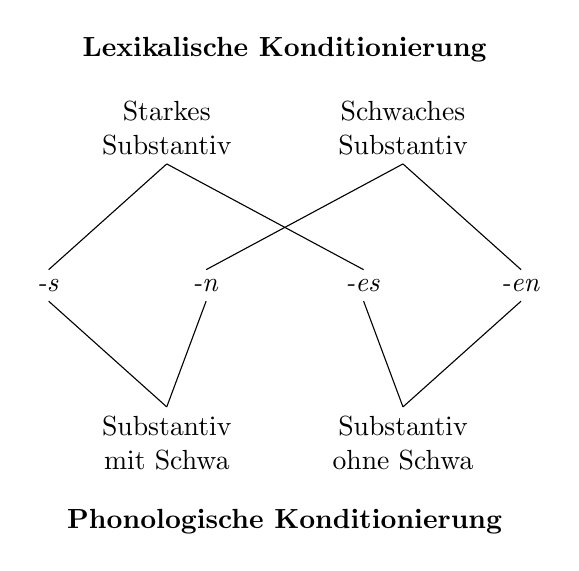
\begin{tikzpicture}[every text node part/.style={align=center}]

    \node (LexKond)     at (3,6) {{\textbf{Lexikalische Konditionierung}}};
    \node (StrkSubst)   at (1.5,5) {Starkes\\Substantiv};
    \node (SchwSubst)   at (4.5,5) {Schwaches\\Substantiv};

    \node (SuffS)       at (0,3) {\textit{-s}};
    \node (SuffN)       at (2,3) {\textit{-n}};
    \node (SuffEs)      at (4,3) {\textit{-es}};
    \node (SuffEn)      at (6,3) {\textit{-en}};

    \node (SubstMSchwa) at (1.5,1) {Substantiv\\mit Schwa};
    \node (SubstOSchwa) at (4.5,1) {Substantiv\\ohne Schwa};
    \node (PhonKond)    at (3,0) {{\textbf{Phonologische Konditionierung}}};

    \draw (SuffS.south)  -- (SubstMSchwa.north);
    \draw (SuffS.north)  -- (StrkSubst.south);
    \draw (SuffEs.south) -- (SubstOSchwa.north);
    \draw (SuffEs.north) -- (StrkSubst.south);

    \draw (SuffN.south)  -- (SubstMSchwa.north);
    \draw (SuffN.north)  -- (SchwSubst.south);
    \draw (SuffEn.south) -- (SubstOSchwa.north);
    \draw (SuffEn.north) -- (SchwSubst.south);
  \end{tikzpicture}
  \caption{Konditionierungen beim hypothetischen Genitiv-Morphem}
  \label{fig:lexikonregeln049}
\end{figure}

\begin{table}[!htbp]
  \begin{tabular}{llll}
 \lsptoprule
    \textbf{Kasus} & \textbf{Löwe} & \textbf{Wort} & \textbf{Mutter} \\
    \midrule
     \textbf{Nominativ} & Löwe-n & Wört-er   & Mütter   \\
     \textbf{Akkusativ} & Löwe-n & Wört-er   & Mütter   \\
     \textbf{Dativ}     & Löwe-n & Wört-er-n & Mütter-n \\
     \textbf{Genitiv}   & Löwe-n & Wört-er   & Mütter   \\
    \lspbottomrule
  \end{tabular}
  \caption{Plural von \textit{Löwe}, \textit{Wort}, \textit{Mutter}}
  \label{tab:lexikonregeln050}
\end{table}

Ein weiteres Argument betrifft die funktionale Ebene.
Bleiben wir bei dem Beispielwort \textit{Löwe}, nehmen \textit{Wort} und \textit{Mutter} hinzu und sehen uns den Plural in Tabelle~\ref{tab:lexikonregeln050} an.
\textit{Löwe} bildet alle Formen des Plurals mit dem Morph \textit{-n}.
\textit{Wort} bildet alle Formen mit \textit{-er} und Umlaut, und nur im Dativ wird zusätzlich \textit{-n} angehängt.
\textit{Mutter} bildet die Pluralformen überhaupt nicht durch Anhängen eines Morphs, sondern nur durch Umlaut, wobei der Dativ zusätzlich durch \textit{-n} markiert ist.
In dieser Situation müssen wir fragen, welche Markierungsfunktion die Morphe tatsächlich haben.
Im Prinzip wird ganz offensichtlich bei Wörtern wie \textit{Löwe} durch \textit{-n} nur der Plural und nicht etwa der Kasus markiert.
Bei \textit{Wort} kann man \textit{-er} als Pluralmorph und \textit{-n} als Allomorph des Dativ-Morphems identifizieren.
Im Falle von \textit{Mutter} wird es schwieriger, weil der Plural nicht wirklich mittels eines Morphs markiert wird.
In vielen Ansätzen wird an dieser Stelle auch gerne ein (unsichtbares) \textit{Null"=Allomorph} (in der Analyse \zB als $\emptyset$ notiert) des Plural-Morphems angenommen, das seinerseits im Sinne einer grammatischen Konditionierung das umgelautete Allomorph des Lexems fordert, s.\ (\ref{ex:lexikonregeln051}).

\begin{exe}
  \ex{\label{ex:lexikonregeln051} Mütter-$\emptyset$}
\end{exe}

Obwohl dies zwar eine theoretisch zulässige Analyse ist, sinkt der explanatorische Gehalt des Morphembegriffs damit deutlich.
Noch schwieriger wird die Situation, wenn zu \textit{Löwe} die Formen des Singulars hinzugezogen werden, und das Paradigma vollständig betrachtet wird.
Außer dem Nominativ Singular lauten nämlich alle Formen des Wortes \textit{Löwe-n}.
Es ist in Anbetracht des gesamten Paradigmas nicht besonders plausibel, \textit{-n} im Plural als Allomorph des Plural-Morphems zu analysieren, weil die eigentliche Markierungsfunktion des \textit{-n} hier die zu sein scheint, den Nominativ Singular allen anderen Formen gegenüberzustellen (vgl.\ auch Seite~\pageref{abs:morphe015}).
Andernfalls müsste man annehmen, dass \textit{-n} in den Singularformen einmal als Allomorph des Akkusativ-Morphems auftritt, einmal als Allomorph des Dativ-Morphems und einmal als Allomorph des Genitiv"=Morphems.

\index{Markierungsfunktion}

Zusammenfassend kann man sagen, dass ohne Zweifel in einigen Fällen Markierungsfunktionen wie Genitiv (nur im Singular, \zB bei \textit{Wort-es}) oder Dativ (nur im Plural, \zB bei \textit{Mütter-n}) oder aber Plural (\zB bei \textit{Wört-er} oder \textit{Mütter}) durch bestimmte formale Mittel angezeigt werden.
Allerdings haben die formalen Mittel nicht immer die Gestalt eines Morphs, \zB der Plural-Umlaut in \textit{Mütter}.
Außerdem ist die explizite und differenzierte Markierung des Kasus sehr eingeschränkt:
Außer manchen Genitiven im Singular und nahezu allen Dativen im Plural wird Kasus am Substantiv nicht markiert.
Man müsste also in den meisten Fällen ein Null-Allomorph für Kasus annehmen.
Die Kasus-Morpheme stünden damit auf einer sehr schmalen Basis aus tatsächlich vorkommenden Morphen.
Letztlich scheint es bei einigen Substantiven (\zB \textit{Löwe}) so zu sein, dass das einzige auftretende Morph eine ganz andere Funktion hat, als explizit Kasus und\slash oder Numerus zu markieren.
Das \textit{-n} hat hier vereinfacht gesagt eine negative Markierungsfunktion, indem es genau eine Kasus-Numerus-Markierung (Nominativ Singular) ausschließt.
Mehr dazu findet sich in Kapitel~\ref{sec:nominalflexion}.

\Np

Es gibt also gute Gründe, warum wir im weiteren Verlauf davon absehen, die Morphem\slash Allomorph-Terminologie zu verwenden.
Dies soll uns natürlich nicht daran hindern, nach den Markierungsfunktionen von Morphen in Wortformen zu fragen.
Wir beziehen uns dabei nur nicht auf die (für das Deutsche überwiegend) unnötig abstrakte Einheit des Morphems.

\end{Vertiefung}

\Uebungen

\Uebung[\tristar]{} \label{exc:morphologie01} Bestimmen Sie die Kasus der in [] eingeklammerten Kasusformen in den folgenden Beispielen und überlegen Sie, welche Funktion diese jeweils haben.%
\footnote{Die Markierungsfunktion im engeren Sinne ist natürlich jeweils nur Kasus und ggf.\ Numerus.
Mit Funktion im weiteren Sinn ist hier gemeint, welche strukturbildende Funktion der Kasus in der Gesamtkonstruktion hat.
Vgl.\ dazu Abschnitt~\ref{sec:formundfunktion}.}
Es geht jeweils um die gesamte nominale Gruppe (also Artikel, Adjektiv und Substantiv), weil diese eindeutiger für Kasus markiert ist als das einzelne Substantiv.
Sie müssen nicht unbedingt Merkmale oder genaue Definitionen angeben.
Überlegen Sie vielmehr, ob die Kasus regiert sind (und von welchem Wort), ob sie (informell) einen eigenen Bedeutungsbeitrag haben, ob sie unabdinglich für eine eindeutige Interpretation des Satzes sind, ob die gesamte nominale Gruppe vielleicht weglassbar ist usw.

\begin{enumerate}
  \item {[Mir]} graut vor diesem Spiel.
  \item {[Es]} graut mir vor diesem Spiel.
  \item Sie wollte {[den Ball]} ins Tor schießen.
  \item Alle schauen mit {[großer Freude]} zu.
  \item Das Maskottchen {[der siegreichen Mannschaft]} ist immer dabei.
  \item {[Das Maskottchen]} der siegreichen Mannschaft ist {[eine Löwin]}.
  \item Alexandra träumt von {[der Meisterschaft]}.
  \item {[Den ganzen Tag]} hat Theo über Frauenfußball gesprochen.
  \item Der Ball läuft gut auf {[dem Rasen.]}
  \item Der Ball rollt auf {[den guten Rasen]}.
  \item {[Wir]} geben {[den Vereinen]} gerne {[unsere Unterstützung]}.
  \item Wir fahren {[dem Trainer]} gerne {[die Ausrüstung]} nach Duisburg.
  \item {[Dieses Jahr]} fahren wir zu mindestens drei Spitzenspielen.
\end{enumerate}

\Uebung[\tristar]{} \label{exc:morphologie02} Versuchen Sie, einzelne Morphe in den folgenden Verbformen abzutrennen (also eine morphologische Analyse durchzuführen).
Liegt beim Stamm ein Ablaut oder Umlaut vor?
Überlegen Sie, welche Markierungsfunktionen (1) der Ablaut oder Umlaut und (2) die Affixe haben könnten, ggf.\ indem Sie sie mit den Affixen in anderen Wortformen desselben lexikalischen Wortes vergleichen.

\begin{enumerate}
  \item Er {[legt]} das Amt nieder.
  \item Sie {[legen]} sich schlafen.
  \item Theo behauptete, er {[kenne]} sich mit Fußball aus.
  \item Ich {[nehme]} den Ball an.
  \item Du {[nimmst]} den Ball an.
  \item Die Präsidentin {[legte]} das Amt nicht nieder.
  \item Die Präsidentin hat das Amt nicht {[niedergelegt]}.
  \item Sie {[nahmen]} die Wahl an.
  \item Ich glaube, sie {[nähmen]} die Wahl trotz allem nicht an.
  \item {[Angenommen]} hat die Wahl bisher jeder Kandidat.
  \item Du {[schicktest]} mir ja bereits letzte Woche die besagte Email.
  \item Wir sollen endlich {[aufhören]}.
\end{enumerate}

\Uebung[\twostar]{} \label{exc:morphologie03} Überlegen Sie, was in den folgenden Wortformen Affixe der Wortbildung oder Flexion sein könnten.
Welche statischen Merkmale werden überschrieben bzw.\ welche Merkmale gelöscht oder hinzugefügt?

\begin{enumerate}
  \item Sie hat die Torchance {[versiebt]}.
  \item Wir haben das Mehl {[gesiebt]}.
  \item Man dachte, dieses Schiff könne nie {[untergehen]}.
  \item Ein rechtes {[Unwetter]} zieht über Schweden.
  \item Hast du schon {[bezahlt]}?
  \item Hat jemand die Brötchen {[gezählt]}?
  \item Haben wir den Bericht schon {[geschrieben]}?
  \item {[Geschriebenes]} lebt länger.
  \item Die braune Gefahr {[überzieht]} Europa.
  \item Das {[unzufriedene]} {[Genörgel]} reicht mir jetzt.
  \item {[Wölkchen]} ziehen am Himmel.
  \item Unsere {[Fußballerinnen]} verdienen mehr {[Aufmerksamkeit]}.
\end{enumerate}

